\section{New Horizons -- Future trends in Ocean Science}
\label{sec:future}

The future of maritime exploration is heavily dependent on machinery,
whether autonomous or not. The vast variability in spatial and
temporal scales that need to be explored has not and will unlikely not
change in the foreseeable future. Consequently, the use of automation
to replace human presence or even its extension, will require robotic
platforms, a diverse range of sensors and control and analysis
algorithms which can stitch a more incisive picture of the oceanic
environment. To do so, it becomes critical to view a patch of the
ocean across spatial and temporal scales to view processes from the
large to connect with the small (macro to micro). We believe such a
patch should be at the meso-scale with coordinated observations
starting from space based, to aerial, surface and underwater to
discern the processes in the upper water-column so crucial for our
understanding of what sustains life on earth.

Fig. \ref{fig:inverse} visually provides such a perspective. Starting
with the \smle, ocean surface observations can be generated with a
\emph{hyper-synoptic} view of the upper water-column at about 10,000
km\textsuperscript{2} in one snap-shot, with a platform moving in the
order of 15,000 knots, with 'higher' resolution data from
\emph{super-synoptic} UAVs making atmospheric and surface measurements
covering $\sim 1000's$ km\textsuperscript{2} flying at 40--60
knots. Closer in and \emph{in-situ}, potentially synoptic measurements
can be made by ASV's on the surface which can make air/sea flux
measurements, covering potentially $\sim 100's$ km\textsuperscript{2} at
potential 2--10 knots speed. Even higher micro-structure measurements
can then be augmented by AUVs with added in-situ imaging and
water-sampling at the $\sim 10's$ km\textsuperscript{2} scale while
moving through the water column between 1--4 knots. Together this
inverse observational pyramid, forms a cohort of platforms with the
sensors they carry, to detect, track and examine features from space,
all the way to the micro-organisms that inhabit those features.

\begin{figure}[!h]
  \centering
  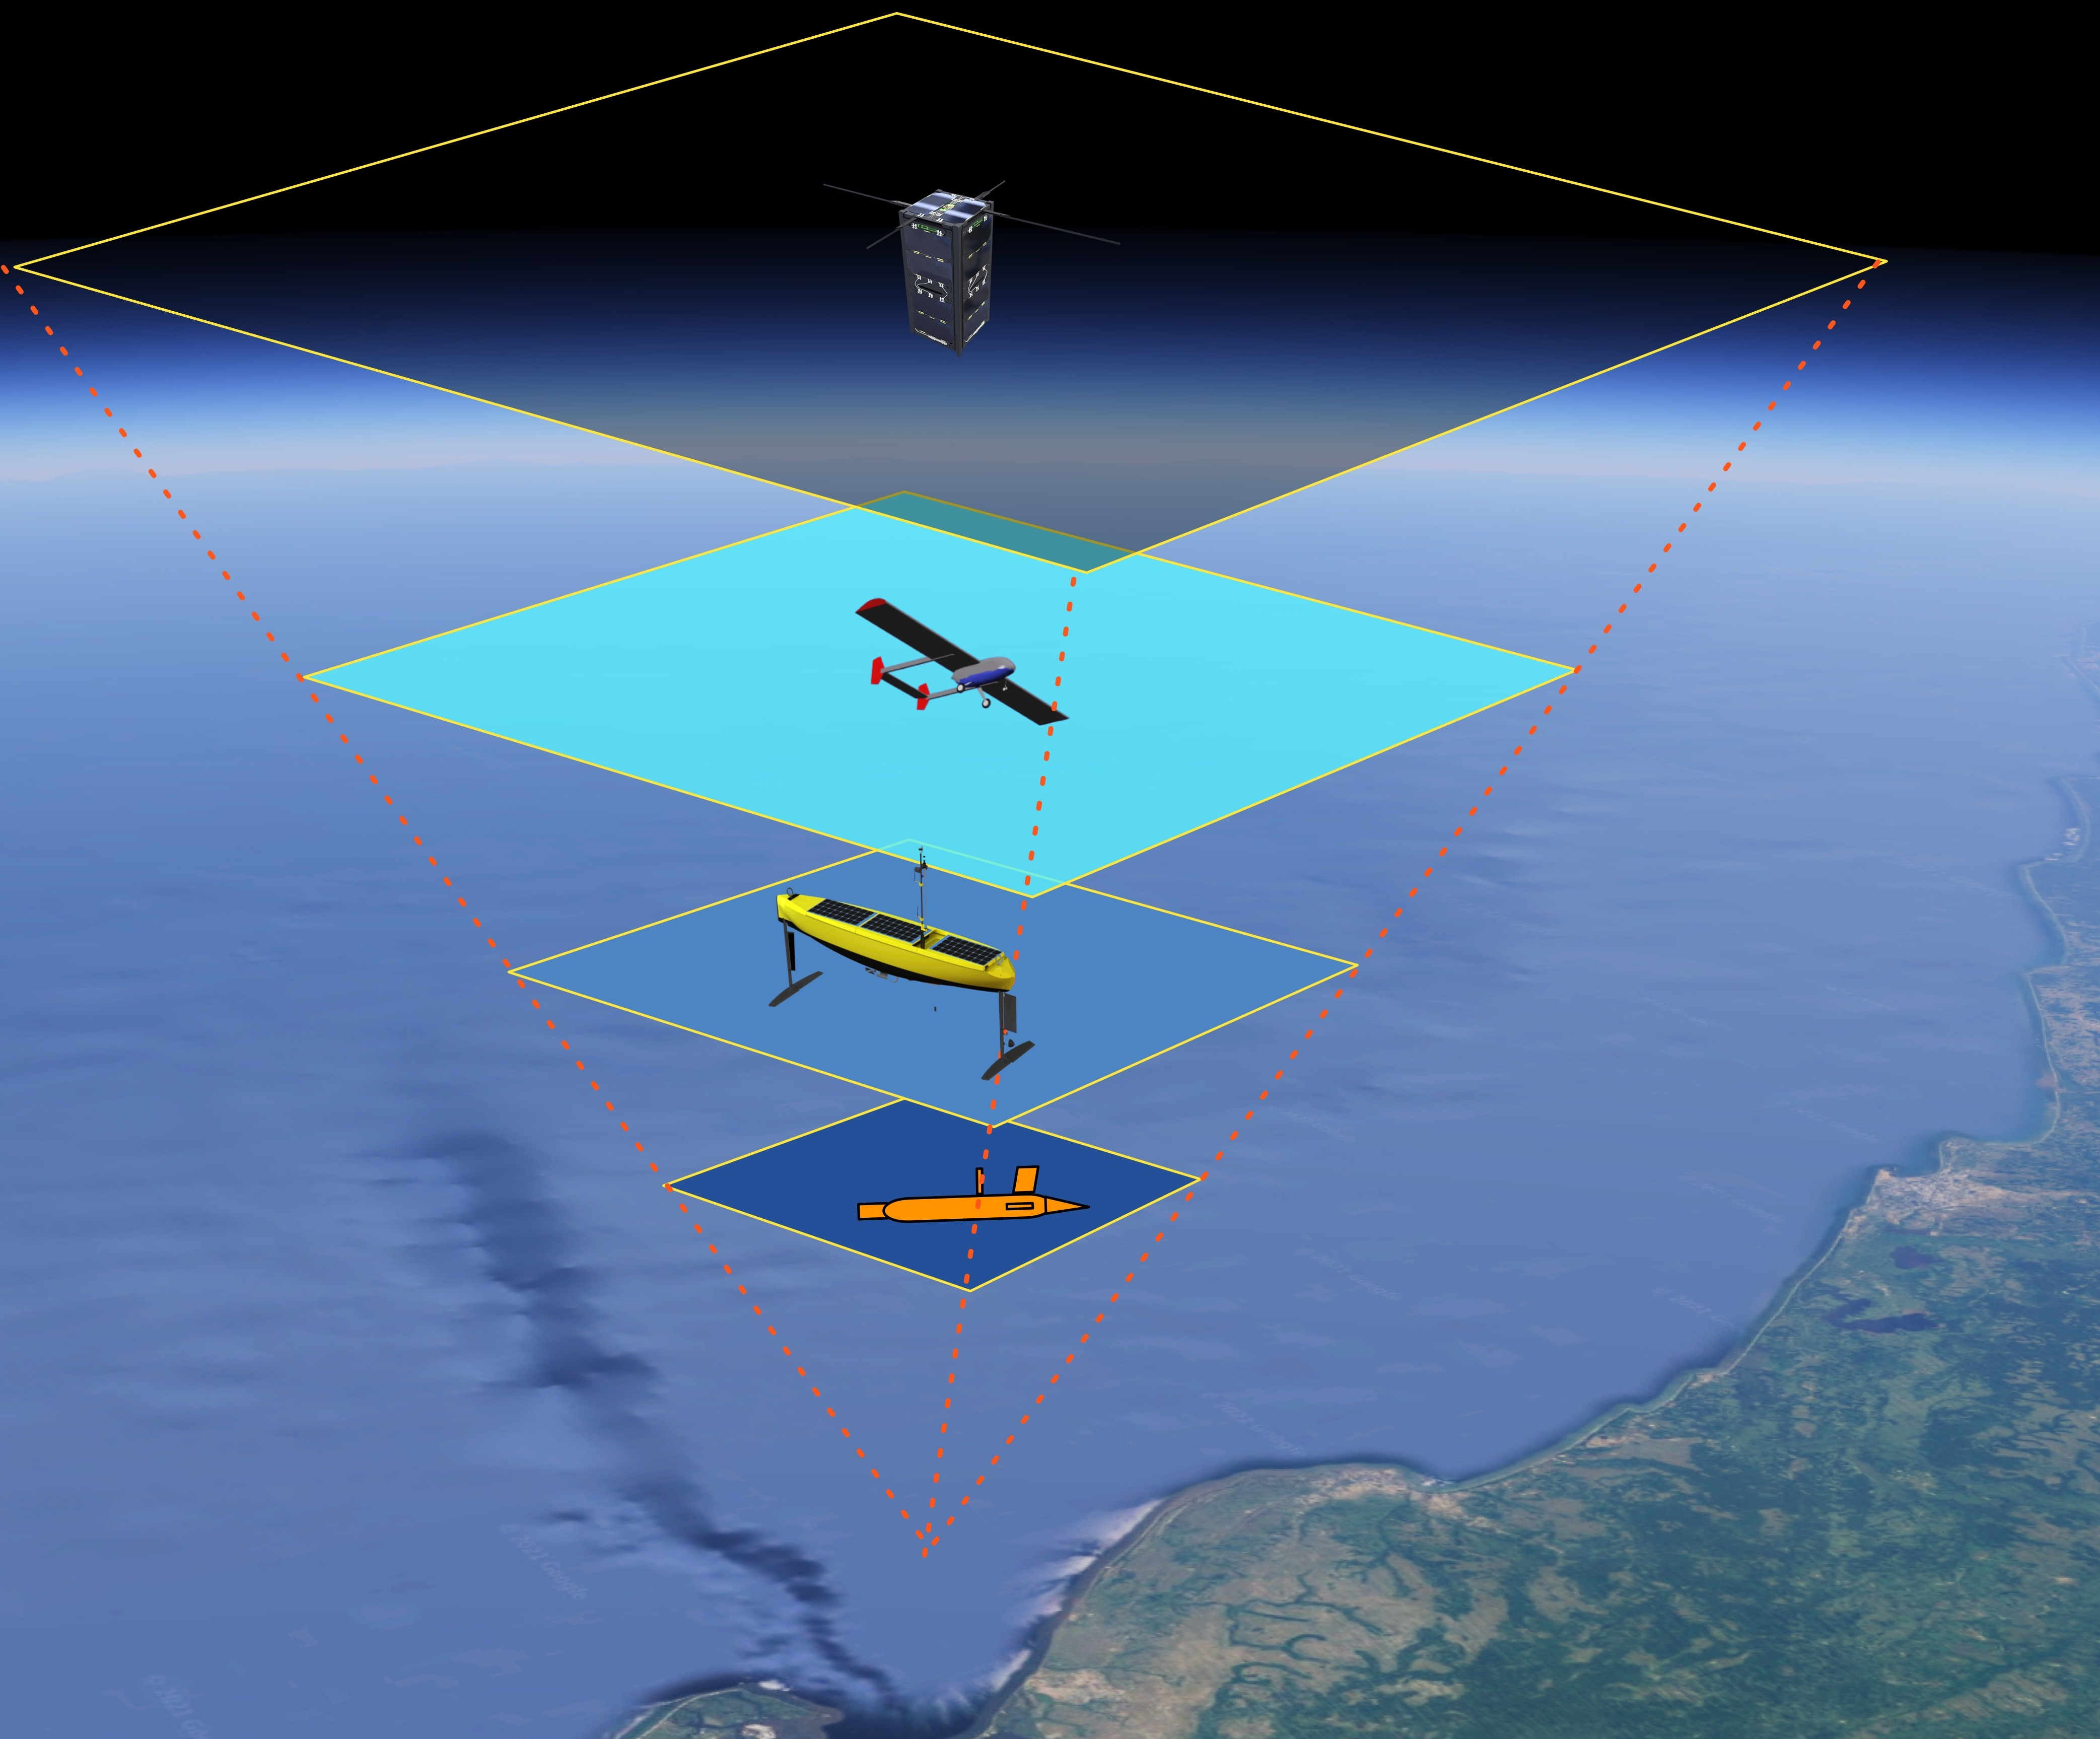
\includegraphics[width=0.9\textwidth]{fig/inverse-pyramid.jpg}
  \caption{Using multi-domain platforms from space, aerial, surface
    and underwater vehicles to observe a patch of the coastal ocean is
    critical to how we can make measurements across the variability in
    spatial and temporal scales. This \textsf{inverse pyramid of
      observational} capability will provide the necessary means to
    discern the bio-geophysical changes in the upper ocean, key to
    human life on Earth.}
  \label{fig:inverse}
\end{figure}

Each platform brings a range of capabilities, from observing at very
large spatial scales via space remote sensing, to making fine scale
measurements in the water column at far slower speeds with AUVs
in-situ. Coordination of these platforms is not necessary about
managing swarming or optimal control behaviors, but more about
ensuring that measurements can be made at approximately the
region/area/volume in as adaptive way as necessary. The expense of
operating such platforms can then work in a dynamic that allows for a
gradated response which use (space or aerial) remote sensing to spot a
feature of interest, which then result in an 'event response'
situation, which can bring to bear more expensive, in terms of
human-aided deployment costs, in-situ assets like ASVs and
AUVs. Aerial platforms can then be used to scour a larger surface area
and direct the deployment of slower moving ASVs and AUVs in targeted
areas. These platforms in turn, can then use onboard adaptive control
to further refine their observations to generate the necessary
fine-scale measurements that science requires at high-resolution. 

\begin{figure}[!h]
  \centering
  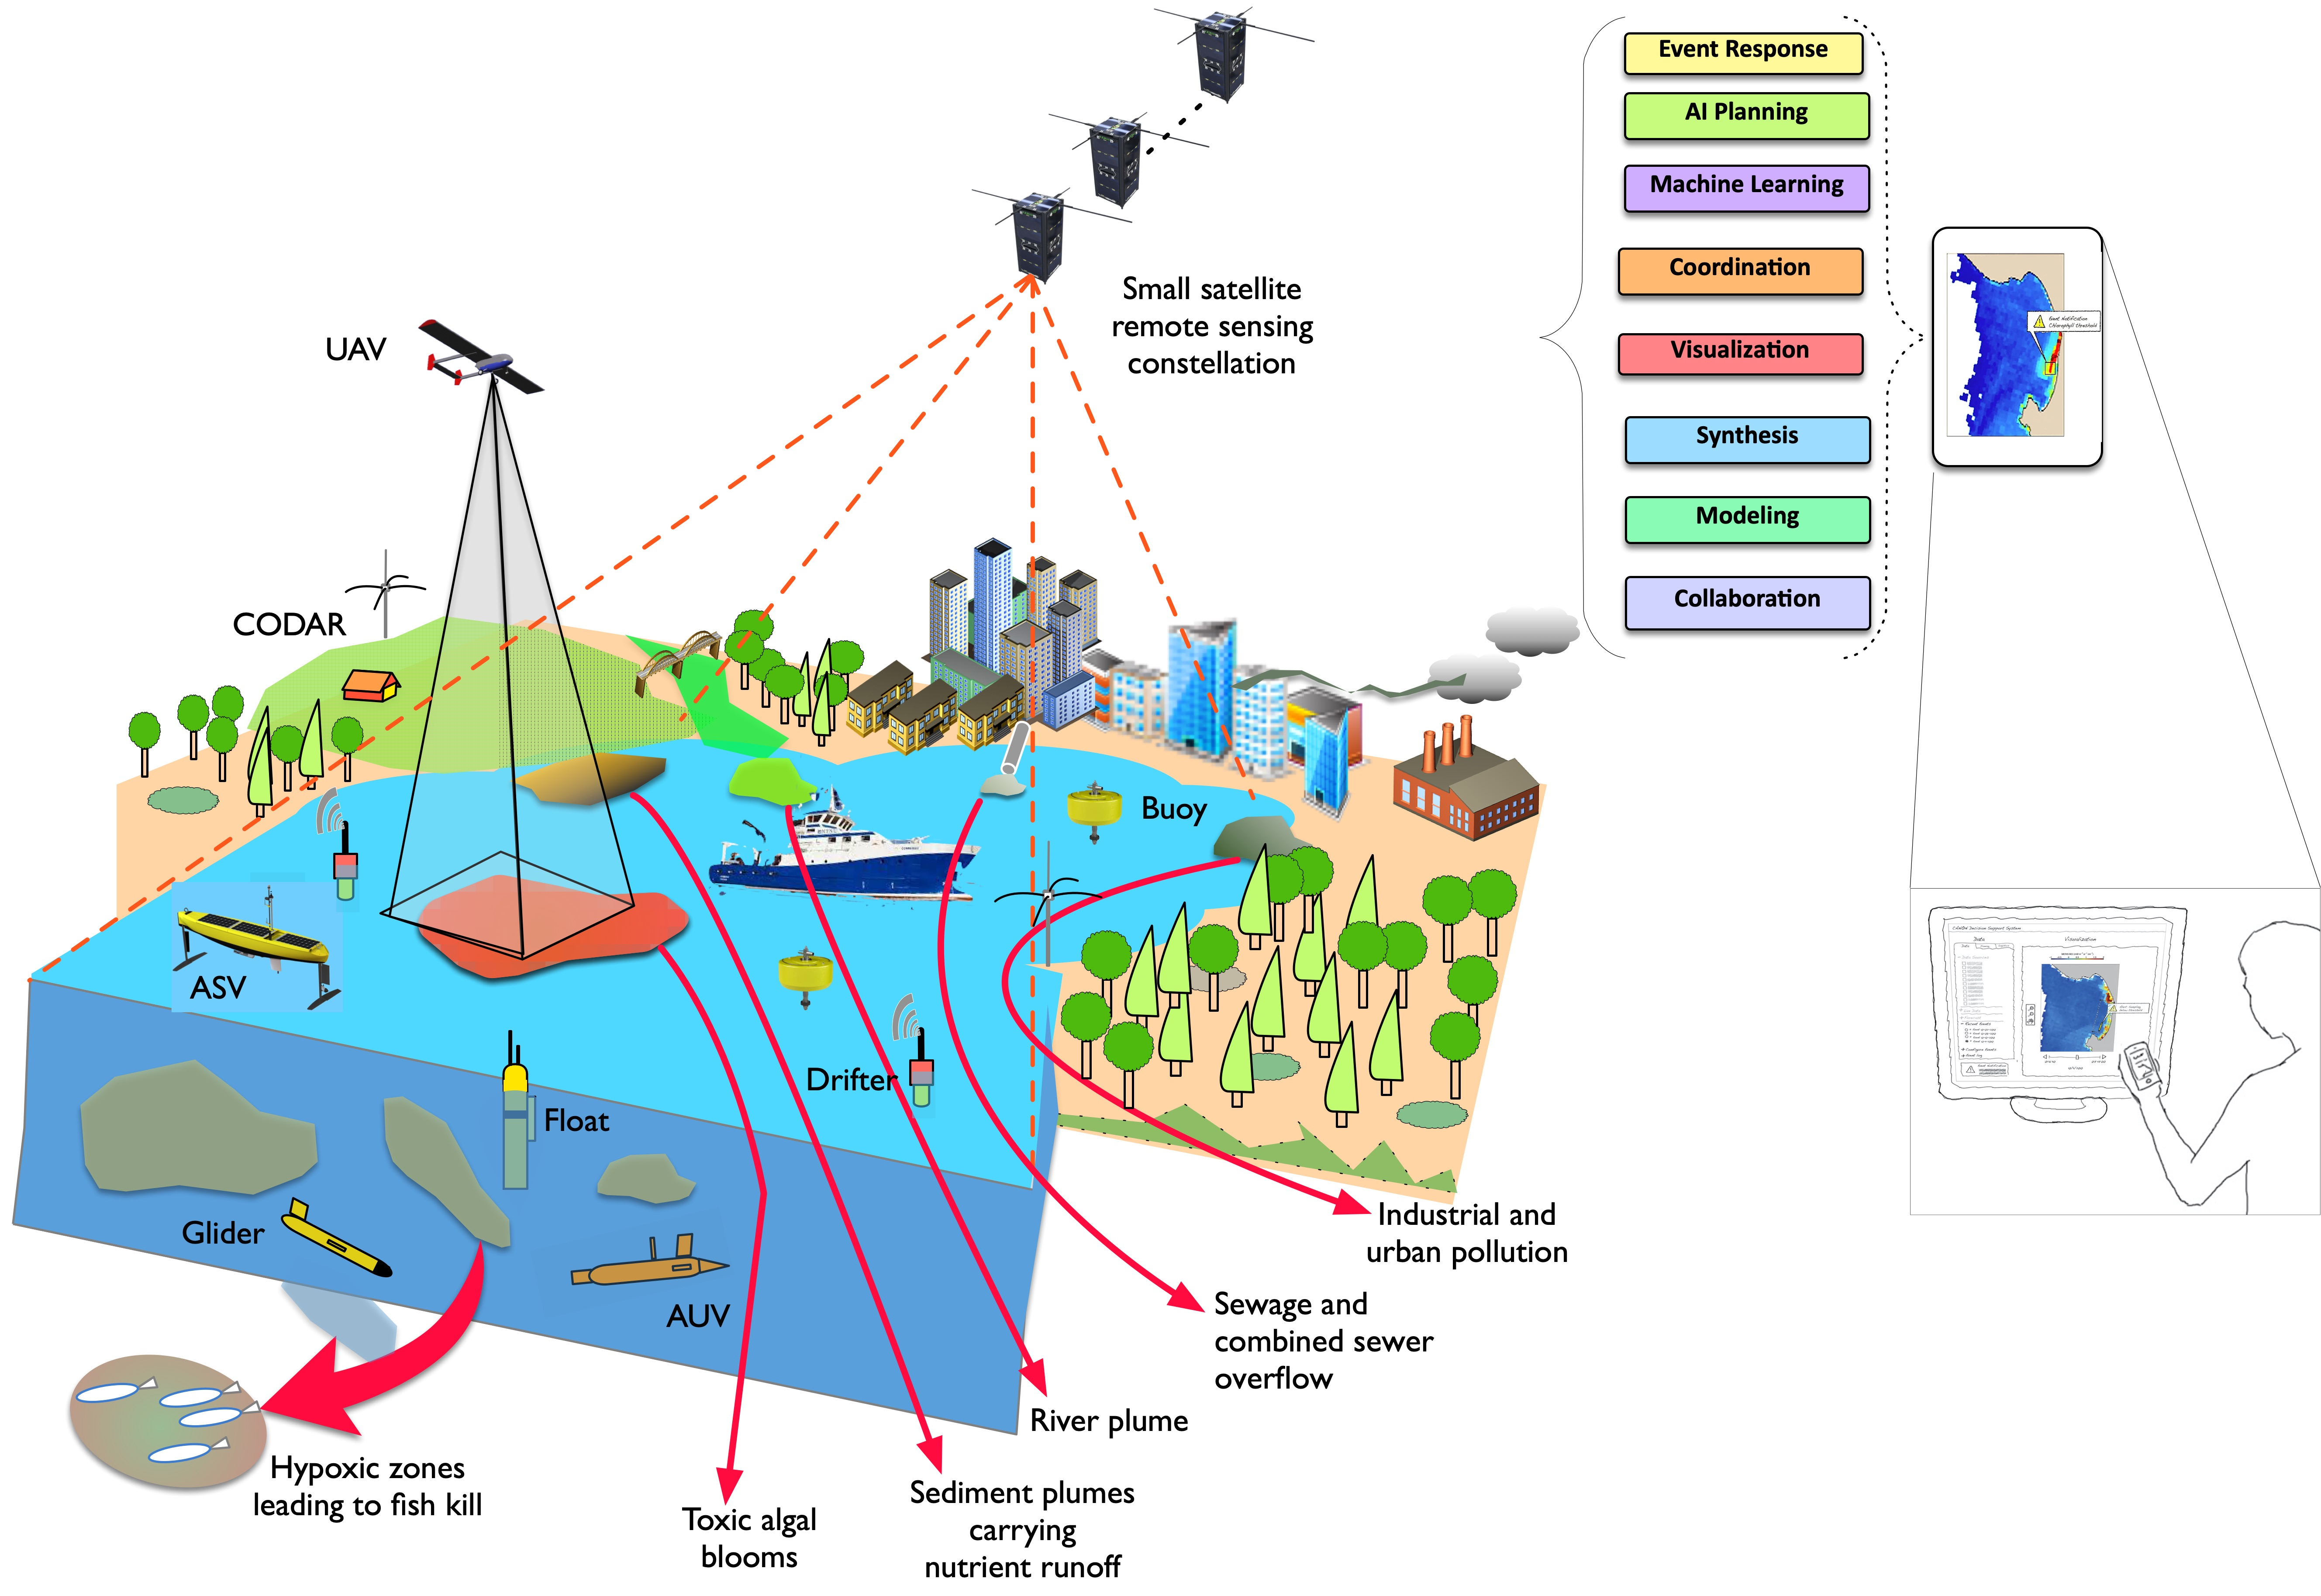
\includegraphics[width=0.9\textwidth]{fig/inverse-pyramid-2.jpg}
  \caption{The backend and embedded computation on robotic vehicles in
  the space, aerial, surface and underwater domains are critical for
  the functioning of the ensemble. The cohort of vehicles will need to
  guided by ocean models, Machine Learned systems to direct them to
  areas of maximal uncertainty, methods to assimilate and fuse data
  from multiple sensors and layered visualization which can show a
  range of possible projections and real-time information.}
  \label{fig:inverse-2}
\end{figure}

This hardware-centric view belies the complexity behind such a likely
scenario since it is backend and embedded software that will actually
provide the necessary means to accomplish the tasks to map dynamic
features in the water-column (Fig. \ref{fig:inverse-2}). Central to
the back end will be data-assimilated ocean models which will
assimilated bio-physical measurements from space and aerial remote
sensing, in addition to digesting continuous measurements from
moorings, buoys, drifters, floats and glider lines to generate
uncertainty maps which can target powered robotic vehicles like ASVs
and AUVs to adaptively sample the water column in high resolution
\cite{berget18,fossum18,fossum18b,fossum19b,fossum21}.


% This could be the core of the m/s -- a look ahead to what we think the
% contributions of AI and Robotics can do, leveraging networked vehicle
% technologies, given large spatial extents to be sampled. 

\begin{enumerate} 
\kc{
\item Implications of the use of robotic vehicles -- plusses and
  challenges. The role of vehicles in space, aerial, surface and
  underwater environments

\item how new generations of spacecraft (incl. SmallSats) could alter
  the landscape — e.g. our pitch to Audacious
  
\item How AI/ML can tie the needs of observational requirements and
  alleviate the issue of space/time and understanding spatio-temporal
  cause-effect relationships

\item The use of robots in security and surveillance. Legal implications
  related to use of robotic vehicles in such domains. 
}
\end{enumerate}

